\documentclass[11pt]{article}

\usepackage[margin=1.2in, a4paper]{geometry}

\usepackage[utf8]{inputenc}

\usepackage{setspace}  % set spacing

\setstretch{1.25}  %stretch line space to multiple x

\usepackage[dvipsnames,table, xcdraw]{xcolor}
% If you use beamer only pass "xcolor=table" option, i.e. \documentclass[xcolor=table]{beamer}

\usepackage{shadowtext}

\usepackage{indentfirst} % indent the first paragraph of each section

\usepackage{float} %determine the position of figures in the document

\usepackage{tabularx} % extra features for tabular environment

\usepackage{amsmath, amsfonts, amssymb}  % improve math presentation

\usepackage{blkarray, bigstrut}

\usepackage{makecell}

\usepackage{mathtools}
\DeclarePairedDelimiter\ceil{\lceil}{\rceil}
\DeclarePairedDelimiter\floor{\lfloor}{\rfloor}



%++++++++++++++++++++++++++++++++++++++++++++++++++++++++++++++++

\usepackage{graphicx} % takes care of graphic including machinery

\graphicspath{{images/}}

%++++++++++++++++++++++++++++++++++++++++++++++++++++++++++++++++



\usepackage{caption}

\usepackage{subcaption}

\usepackage{tikz}

\usepackage{lipsum,lmodern}

\usepackage[most]{tcolorbox}

\usetikzlibrary{trees}  %add binary trees

\usetikzlibrary {positioning}

\usepackage[final]{hyperref} % adds hyper links inside the generated pdf file

\hypersetup{
	colorlinks=true,       % false: boxed links; true: colored links
	linkcolor=blue,        % color of internal links
	citecolor=blue,        % color of links to bibliography
	filecolor=magenta,     % color of file links
	urlcolor=blue         
}

\usepackage{blindtext}

\usepackage{dirtytalk} %quotation marks


%********************************

%Bibliography

\usepackage[backend=biber,  style=alphabetic,  sorting=ynt]{biblatex}

\addbibresource{../../Mybib.bib}


%********************************


\usepackage{fancyhdr}

\pagestyle{fancy}

\fancyhf{}

\lhead{\footnotesize {Mathematical Statistics} }
\rhead{\footnotesize { } }
\cfoot{- \thepage \ -}

\title{\vspace{-90pt} 


%**************************************************

% Title Part
\textbf  {Peer-graded Assignment} }
\author{Cui, Xiaolong(Larry)}
\date{\today}


%*************************************************

\begin{document}

%\maketitle

\thispagestyle{plain}

%*************************************************

\begin{figure}[H] %[!tbp]
  \begin{subfigure}{0.3\textwidth}
    
\includegraphics[width=\textwidth]{uol}
    %\caption{Flower one.}
    %\label{fig:f1}
  \end{subfigure}
  \hfill
  \begin{subfigure}{0.3\textwidth}
    \includegraphics[width=\textwidth]{goldsmiths}
    %\caption{Flower two.}
    %\label{fig:f2}
  \end{subfigure}
  %\caption{My flowers.}
\end{figure}

%****************************************************

\begin{flushright}

\footnotesize {Sept. 15,   2021}
\end{flushright}

\begin{center}
\textbf{Stirling's Formula to De Moivre \& Laplace Theorem} \\
\footnotesize {Study Notes $ | $ Written by Larry Cui}
\end{center}

%***************************************************

\begin{abstract}
Stirling formula and De Moivre Laplace theorem are important intermediate steps toward the central limit theorem.  In many undergraduate statistics textbooks,  however,  step by step proof is often omitted,  which sometimes poses quite a huge challenge to students who want to fully understand the logic behind the formulas.  This note is trying to fill the gap between unusually looking equations and the proofs behind them.  During the process of writing this note,  I referred frequently to \cite{balazs2014stirling} and Jacek Cichon's "Stirling Approximation Formula",  to whom a huge debt is owed.
\end{abstract}


%***************************************************

\setcounter{figure}{0}

\vspace{10pt}


\section {\large Stirling's Formula}


Stirling's formula is necessary for the proof of De Moivre Laplace Theorem.  It's an approximation of the n factorial:

\begin{tcolorbox} 
[colback=blue!5!white,  colframe=blue!75!black,  title= {\textbf{
Stirling's Formula
} }]

$$ n! \approx \sqrt{ 2 \pi n} \left(  \frac{n}{e} \right) ^n $$

\end{tcolorbox}


\section {\large A Rough Estimate}

If we take  logarithm of $n!$,  the product of \say {$1 \cdot 2 \cdot 3 \cdots n$} becomes the sum of logarithms (let's name it as \say { $S(n)$ } ),  i.e.,  $ S(n) = \ln 1 + \ln 2 + \cdots + \ln n$.   A straight forward comparisons below:

\begin{figure}[H] 
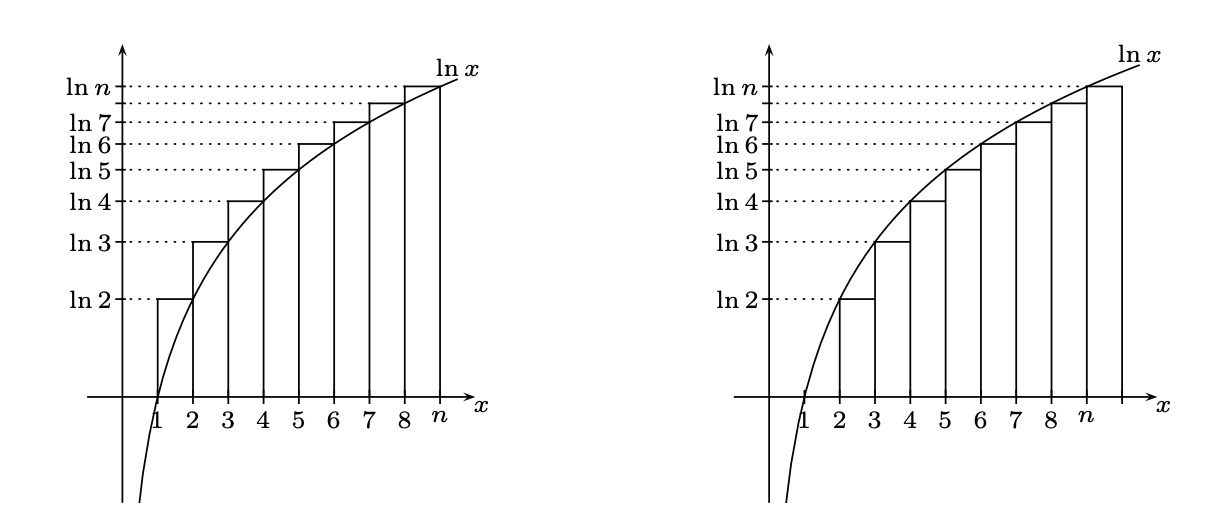
\includegraphics [scale = 0.53] {comparison} %[width=\textwidth]
\centering
\caption{$S(n)$ vs.  $\ln x$ }
\label{fig:f1}
\end{figure}

We can directly derive the following bounds:

\begin{equation}
 \int^{n}_{1} \ln x dx \leqslant  S(n) \leqslant \int ^{n+1} _ {1} \ln x dx
\end{equation}


Integrate the left side of the above equation,  we have 
$$ \int ^n _1 \ln x dx = (x \ln x - x) \bigg \rvert ^n _1 = n \ln n - (n - 1) $$

Integrate the rigth side gives us
$$ \int ^{n+1} _ {1} \ln x dx =  (n+1) \ln (n+1) - n $$

We have new equation from eq.(1) as
$$ \ln \frac {n^n}{e^{n-1}} \leqslant \ln n! \leqslant \ln \frac{(n+1)^{n+1}}{e^n} $$ 
$$ \frac {n^n}{e^{n-1}} \leqslant n! \leqslant  \frac{(n+1)^{n+1}}{e^n} $$

Take a second look at the right side of the above equation,  we can simplify it
$$
\begin{aligned}[t]
\frac{(n+1)^{n+1}}{e^n} 
 	&= \left( \frac{n+1}{e} \right) ^n  (n+1) \\
 	&= \left( \frac{n}{e} \cdot \frac{n+1}{n} \right) ^n (n+1) \\
 	&= \left( \frac{n}{e} \right) ^n \cdot \left( 1 + \frac{1}{n} \right) ^n (n+1)
\end{aligned}\\
$$
as $n \to \infty$,  $\displaystyle \left( 1 + \frac{1}{n} \right) ^n = e$,  the right side becomes $ \displaystyle e(n+1) \left( \frac{n}{e} \right) ^n$,  we have a shorter form of eq. (1) as
$$ e \left( \frac{n}{e} \right) ^n \leqslant n! \leqslant e(n+1) \left( \frac{n}{e} \right) ^n $$
which is saying that 
\begin{equation}
n! = f(n) \left( \frac{n}{e} \right) ^n
\end{equation}
for a function $f(n)$ where $ e \leqslant f(n) \leqslant e(n+1) $.


\section {\large Finding Constant C}

We re-arrange eq. (2) by dividing both sides with $ \displaystyle \sqrt{2n} \left( \frac{n}{e} \right) ^n $:

$$ \displaystyle  \frac {n!}  { \sqrt{2n}  \left( \frac{n}{e} \right) ^n } = \frac {f(n)} { \sqrt{2n} } $$
now we need to find a limit C (if there's one) of the left side when n approaches to 0,  then we get our result for                 $\displaystyle n! \approx C  \sqrt{2n}  \left( \frac{n}{e} \right) ^n $.


\subsection{\normalsize The Integration of $ \displaystyle \int \sin ^n x  \, dx$}

We start from the integration of $\sin^n x \, dx$: 
$$
\begin{aligned}[t]
\int \sin ^n x \, dx
    &= \int \sin ^{n-1} x \sin x \, dx\\
    &= - \sin ^{n-1} x \cos x + \int (n-1) \sin ^{n-2} x \cos ^2 x \, dx \\
    &= - \sin ^{n-1} x \cos x + \int (n-1) \sin ^{n-2} x (1 - \sin ^2 x)  \, dx \\
    &= - \sin ^{n-1} x \cos x + \int (n-1) \sin ^{n-2} x \, dx -  \int (n-1)  \sin ^n x \, dx \\
n \int \sin ^n x \, dx &= - \sin ^{n-1} x \cos x + (n-1) \int \sin ^{n-2} x \, dx \\
\end{aligned}\\
$$
so we have, 
$$
\begin{aligned}[t]
\int \sin ^n x \, dx 
	&= - \frac{1}{n} \sin ^{n-1} x \cos x + \frac{n-1}{n} \int \sin ^{n-2} x \, dx \\
\end{aligned}\\
$$
If we evaluate from $\displaystyle 0 \sim \frac{\pi}{2}$,  the above equation reduces to
$$ \int _0 ^{\pi/2} \sin ^n x dx = \frac{n-1}{n} \int _0 ^{\pi/2} \sin ^{n-2} x dx $$

Let $S$ be the integration sum,  we need two different equations to address two situations,  one for even and one for odd:

(a) for $\displaystyle n=k $,
$$
\begin{aligned}[t]
S_{even} 
	&= \int _0 ^{\pi /2} \sin ^{2k} x \, dx \\
	&= \frac{2k-1}{2k} \cdot \frac{2k-3}{2k-2} \cdots \frac{1}{2} \cdot \int _0 ^{\pi/2} \sin ^0 x \, dx \\
	&= \frac{\pi}{2} \prod _{k=1} ^{n/2} \frac{2k-1}{2k} \\
\end{aligned}\\
$$

(b) for $\displaystyle n=2k+1$,  
$$
\begin{aligned}[t]
S_{odd} 
	&= \int _0 ^{\pi /2} \sin ^{2k+1} x \, dx \\
	&= \frac{2k}{2k+1} \cdot \frac{2k-2}{2k-1} \cdots \frac{2}{3} \cdot \int _0 ^{\pi/2} \sin ^1 x \, dx \\
	&= \prod _{k=1} ^{(n-1)/2} \frac{2k}{2k+1} \cdot (-\cos x) \bigg \rvert _0 ^{\pi/2} \\
	&= \prod _{k=1} ^{(n-1)/2} \frac{2k}{2k+1} \\
\end{aligned}
$$

\subsection{\normalsize Wallis Product Formula}

\begin{tcolorbox} 
[colback=blue!5!white,  colframe=blue!75!black,  title= {\textbf{
Wallis Formula
} }]

$$ \prod _{n=1} ^{\infty } \frac{2n}{2n-1} \frac {2n}{2n+1} = \frac{\pi}{2} $$

\end{tcolorbox}

The left side of Wallis formula is actually $\displaystyle \frac{\pi}{2} \cdot \frac {S_{odd}}{S_{even}}$ for $x \in (0,  \pi/2)$.  If we can prove that  $\displaystyle \frac {S_{odd}}{S_{even}} = 1 $ as $ n \to \infty$,  we are done with the proof.  First of all,  we know that
$$ 0 < \sin ^{2k+2} x < \sin ^{2k+1} x < \sin ^{2k} x $$
$$ 0 < S_{2k+2} < S_{2k+1} < S_{2k} $$
divide by $S_{2k}$ on each term,  we have 
$$ 0 < \frac{S_{2k+2}}{S_{2k}} < \frac{ S_{2k+1} } {S_ {2k}} < 1 $$
Because $\displaystyle \lim _{k \to \infty} \frac{S_{2k+2}}{S_{2k}} = \lim _{k \to \infty} \frac{2k+1}{2k+2} = 1  $,  we can apply the squeeze theorem here that
$$ 1 < \frac{S_{2k+1}}{S_{2k}} < 1 \text {\ \ \ \ when } k \to \infty $$
$$ \text {so \  \ } \frac {S_{odd}}{S_{even} }= 1 \text {\  \  \  \  when} k \to \infty $$

\subsection{\normalsize Next Step}
Now we have all tools we need to crack down the constant $C$.  First,  let's re-write the Wallis formula in a compact way:
$$
\begin{aligned}[t]
 \prod _{n=1} ^{n } \frac{2n}{2n-1} \frac {2n}{2n+1}
    &= 2^{2n} (n!)^2  \prod _{n=1} ^{n } \frac{1}{2n-1} \frac{1}{2n+1}\\
    &= 2^{2n} (n!)^2 \cdot \frac{2 \cdot 4 \cdots 2n}{(2n)!} \cdot \frac{2 \cdot 4 \cdots 2n}{(2n+1)!}\\
    &= \frac{2^{2n} (n!)^2 2^{2n} (n!)^2} {((2n)!)^2 (2n+1)}\\
\end{aligned}\\
$$
so
\begin{equation}
 \prod _{n=1} ^{n } \frac{2n}{2n-1} \frac {2n}{2n+1} = \frac{2^{4n} (n!)^4} {((2n)!)^2 (2n+1)}
\end{equation}

Since we pick $C$ so $\displaystyle n! \approx C  \sqrt{2n}  \left( \frac{n}{e} \right) ^n $,  the equation still holds if we substitute $n$ by $2n$:  $\displaystyle (2n)! \approx C  \sqrt{4n}  \left( \frac{2n}{e} \right) ^{2n} $.  Now we use C terms instead of $n!$ and $2n!$ and re-write eq.(3) as follows:
$$
\begin{aligned}[t]
\frac{2^{4n} (n!)^4} {((2n)!)^2 (2n+1)}
	&= \frac{2^{4n} (C  \sqrt{2n}  \left( \frac{n}{e} \right) ^n ) ^4 } { (C \sqrt{4n} ( \frac{2n}{e} ) ^{2n} ) ^2 (2n+1)} \\
	&= \frac{2^{4n} C^4  4n^2  \left( \frac{n}{e} \right) ^{4n} } { C^2 4n ( \frac{2n}{e} ) ^{4n} (2n+1)} \\
	&= \frac{2^{4n} C^2  n  \left( \frac{1}{2} \right) ^{4n} } { 2n+1} \\
	&= C^2 \frac{n} {2n+1} \\
\end{aligned}\\
$$
from Wallis formula,  we know
$$
\begin{aligned}[t]
\lim _{n \to \infty}  C^2 \frac{n} {2n+1} 
	&= \frac{\pi}{2} \\
C^2 \cdot \frac{1}{2} 
	&= \frac{\pi}{2} \\
C 	&= \sqrt{\pi} \\
\end{aligned} \\
$$


\section{\large Rethink of C}

We've known that Stirling's formula is the limit of $n!$ when $n \to \infty$,  so is the $C$.  However,  if $n$ is not a very large number, what's the boundaries of $C$, i.e., 
$$
? \leqslant   \frac {n!}  { \sqrt{2n}  \left( \frac{n}{e} \right) ^n } \leqslant ?
$$

Let 
$$
a_n =  \frac {n!}  { \sqrt{2n}  \left( \frac{n}{e} \right) ^n } 
\text{ \ \ \ \ and \ \ \ \ }
b_n = \ln a_n
$$
we get the equation of $b_n - b_{n+1}$ as follows:
$$
\begin{aligned}[t]
b_n - b_{n+1}
	&= \ln n! - \frac{1}{2} \ln {2n} - n(\ln n - 1) - \ln (n+1)! + \frac{1}{2} \ln (2n+2) + (n+1)( \ln (n+1) - 1) \\
	&= -\ln \left(n+1 \right) + \frac{1}{2} \ln \left(\frac{n+1}{n} \right) + (n+1)(\ln (n+1)) - n \ln n - 1 \\
	&=  n \ln (n+1) - n \ln n + \frac{1}{2} \ln \left( \frac{n+1}{n} \right) - 1 \\
	&= \left(n + \frac{1}{2} \right) \ln \left( \frac{n+1}{n} \right) -1 \\
\end{aligned} \\
$$

Now we need some techniques from Taylor Series expansion.  First of all,  we use $t= \displaystyle  \frac{1}{2n+1}$ to re-write the above equation as
$$ b_n - b_{n+1} = \frac{1}{2t} \ln \frac{1+t}{1-t} -1 $$
then we use polynomial expansion of $\ln (1+t)$:
$$ \ln (1+t) = t - \frac{t^2}{2} + \frac{t^3}{3} - \cdots =  - \sum _{k=1} ^\infty (-1)^k \frac{t^k}{k} $$
and of $\ln (1-t)$:
$$ \ln (1-t) = -t -  \frac{t^2}{2} - \frac{t^3}{3} - \cdots = - \sum _{k=1} ^\infty \frac{t^k}{k} $$
so
$$
\begin{aligned}[t]
 b_n - b_{n+1} 
 	&= \frac{1}{2t} \left(  - \sum _{k=1} ^\infty (-1)^k \frac{t^k}{k} +  \sum _{k=1} ^\infty \frac{t^k}{k} \right) -1 \\
 	&= \frac{1}{2t} \sum _{k=0} ^\infty \frac{2t^{2k+1}} {2k+1}  -1 \\
	&=  \frac{1}{t} \sum _{k=1} ^\infty \frac{t^{2k+1}} {2k+1} 
\end{aligned}
$$


Because we are constructing $t$ in such a way that no matter what value $n$ takes from positive integers, $t$ will always be positive either,  we know that $d_n$ is decreasing.  

Further,  we look at another feature of $d_n - d_{n+1}$ when we change $t$ back to $n$:
\begin{equation}
\begin{aligned}[b]
 b_n - b_{n+1} 
 	&= \frac{1}{t} \sum _{k=1} ^\infty \frac{t^{2k+1}} {2k+1} \\
	&= (2n + 1) \sum _{k=1} ^\infty \frac{1} {2k+1} \frac{1}{(2n+1)^{2k+1}} \\ 	
	&= \sum _{k=1} ^\infty \frac{1} {2k+1} \frac{1}{(2n+1)^{2k}} \\ 
\end{aligned}
\end{equation}
We can derive two inequality forms from eq. (4):
$$
\begin{aligned}[b]
 b_n - b_{n+1} 
 	&<  \sum _{k=1} ^\infty \frac{1}{3} \frac{1}{(2n+1)^{2k}} \\ 
	&= \frac{1}{3} \frac{1}{(2n+1)^{2}} \cdot \frac{1}{ 1 - \frac {1} {(2n+1)^2} } \\
	&= \frac{1}{12} \frac{1}{n(n+1)} \\
\end{aligned}
$$
and
$$
\begin{aligned}[b]
 b_n - b_{n+1} 
 	&>  \sum _{k=1} ^\infty \frac{1}{(2k+1)^{2k+1}}  \ \ \footnotemark \\ 
\end{aligned}
$$
\footnotetext {I haven't figured out how to simplify the right side of the above equation.}

Observe that (a telescoping sum):
$$ 
\begin{aligned}
b_1 - b_n 
	&= (b_1 - b_2) + (b_2 - b_3) + (b_3 - b_4) + \cdots + (b_{n-1} - b_n) \\
	&< \frac{1}{12} \sum _{m=1} ^{n-1} \frac{1}{m(m+1)} = \frac{1}{12} \left( 1 - \frac{1}{n} \right) \text{\ \ and, } \\
	&>  \sum _{k=1} ^\infty \frac{1}{(2k+1)^{2k+1}} \\
\end{aligned}
$$
hence
$$ b_n > b_1 - \frac{1}{12} \left( 1 - \frac{1}{n} \right) = \frac{11}{12} - \frac{1}{2} \ln 2 + \frac{1}{12n}$$
and
$$ b_n < b_1 - \sum _{k=1} ^\infty \frac{1}{(2k+1)^{2k+1}} = 1 - \frac{1}{2} \ln 2 - \sum _{k=1} ^\infty \frac{1}{(2k+1)^{2k+1}} $$






%++++++++++++++++++++++++++++++++++++++++


\printbibliography [title={Reference}]


%***********************************

\end{document}
